% Provenance (never printed): cycle 3 geography and "La planete Terre"
% (the great physical features of the world: relief, rivers, deserts, ice;
% reading a physical map); see sources/book1/PROVENANCE.md.
% Book 1, grade 4, chapter 3.
\chapter{विश्व का भौतिक मानचित्र}\label{ch:g4:world-physical-map}

सामी और नूर कक्षा के फ़र्श पर दुनिया का एक बड़ा \omterm{def:g2:drawing-to-map:map}{मानचित्र} खोलते हैं और उसके
चारों ओर घुटनों के बल बैठ जाते हैं। यह उन \omterm{def:g2:drawing-to-map:map}{मानचित्रों} जैसा नहीं है जिन्हें वे
जानते हैं। इसमें न देश हैं, न सीमाएँ, न शहर। इसके बदले ज़मीन रंगों में रँगी है:
तटों के साथ और बड़े समतल इलाक़ों में हरा, फिर हल्का पीला, फिर भूरा, और कुछ
जगहों पर लगभग सफ़ेद। \omterm{def:g2:water-on-earth:ocean}{समुद्र} के भी कई नीले रंग हैं: तटों के पास हल्का, और
\omterm{def:g2:water-on-earth:ocean}{महासागरों} में दूर जाते-जाते गहरा और गहरा।

``एशिया का वह हिस्सा सफ़ेद क्यों है?'' नूर पूछती है। ``क्या वह \omterm{def:g4:clouds-rain-snow:precipitation}{हिम} है?'' ठीक-ठीक
नहीं। इस \omterm{def:g2:drawing-to-map:map}{मानचित्र} पर हर रंग बताता है कि ज़मीन कितनी ऊँची है, या \omterm{def:g2:water-on-earth:ocean}{समुद्र} कितना गहरा।

\begin{recall}
\omterm{def:g2:drawing-to-map:map}{मानचित्र} किसी जगह को ऊपर से, छोटा करके दिखाता है; उसकी \omterm{def:g2:drawing-to-map:legend}{संकेत-सूची} उसके रंगों और
चिह्नों को समझाती है (\cref{ch:g2:drawing-to-map})। ज़मीन सात \omterm{def:g3:continents-and-oceans:continent}{महाद्वीपों} में बँटी
है, जो पाँच \omterm{def:g2:water-on-earth:ocean}{महासागरों} के बीच हैं, और \omterm{def:g3:continents-and-oceans:world-map}{विश्व मानचित्र} एक चपटा किया हुआ \omterm{def:g3:continents-and-oceans:globe}{ग्लोब} है
(\cref{ch:g3:continents-and-oceans})। \omterm{def:g1:landscapes-around-us:landform}{पर्वत}, \omterm{def:g1:landscapes-around-us:landform}{पहाड़ियाँ}, \omterm{def:g1:landscapes-around-us:landform}{घाटियाँ} और \omterm{def:g1:landscapes-around-us:landform}{मैदान} \omterm{def:g1:landscapes-around-us:landform}{स्थलरूप}
हैं; \omterm{def:g1:landscapes-around-us:water}{नदियाँ} ऊँची ज़मीन से नीचे \omterm{def:g2:water-on-earth:ocean}{समुद्र} की ओर बहती हैं
(\cref{ch:g1:landscapes-around-us})।
\end{recall}

\section{भौतिक मानचित्र पढ़ना}

कोई जगह कितनी ऊँची है, यह बताने के लिए हमें एक शुरुआती तल चाहिए, जो पृथ्वी पर
हर जगह एक ही हो। हम \omterm{def:g2:water-on-earth:ocean}{समुद्र} का तल लेते हैं।

\begin{definition}[ऊँचाई और समुद्र तल]\label{def:g4:world-physical-map:altitude}
\emph{समुद्र तल}\index{समुद्र तल} \omterm{def:g2:water-on-earth:ocean}{समुद्र} की सतह का औसत तल है, ज्वार और भाटे के
बीच। किसी जगह की \emph{ऊँचाई}\index{ऊँचाई} \omterm{def:g2:water-on-earth:ocean}{समुद्र} तल से उसकी ऊँचाई है, मीटर में।
\omterm{def:g2:water-on-earth:ocean}{समुद्र} के नीचे हम \emph{गहराई} की बात करते हैं: \omterm{def:g2:water-on-earth:ocean}{समुद्र} का तल \omterm{def:g2:water-on-earth:ocean}{समुद्र} तल से कितना
नीचे है।
\end{definition}

\omterm{def:g2:water-on-earth:ocean}{समुद्र} किनारे के किसी शहर की \omterm{def:g4:world-physical-map:altitude}{ऊँचाई} कुछ मीटर होती है। पहाड़ों में कोई गाँव
1\,500 मीटर पर हो सकता है: \omterm{def:g2:water-on-earth:ocean}{समुद्र} के तल से डेढ़ किलोमीटर ऊपर, भले ही वह किसी भी
\omterm{def:g1:landscapes-around-us:water}{तट} से सैकड़ों किलोमीटर दूर हो।

\begin{definition}[उच्चावच]\label{def:g4:world-physical-map:relief}
किसी क्षेत्र का \emph{उच्चावच}\index{उच्चावच} उसकी ज़मीन का आकार है: वह कहाँ ऊँची
है और कहाँ नीची, उसके \omterm{def:g1:landscapes-around-us:landform}{पर्वत}, पठार, \omterm{def:g1:landscapes-around-us:landform}{घाटियाँ} और
\omterm{def:g1:landscapes-around-us:landform}{मैदान}।
\end{definition}

\begin{definition}[भौतिक मानचित्र]\label{def:g4:world-physical-map:physical-map}
\emph{भौतिक मानचित्र}\index{भौतिक मानचित्र} ज़मीन के \omterm{def:g4:world-physical-map:relief}{उच्चावच} और \omterm{def:g2:water-on-earth:ocean}{समुद्र} की गहराई को
रंगों से दिखाता है, \omterm{def:g4:world-physical-map:altitude}{ऊँचाई} या गहराई के हर चरण के लिए एक रंग, और साथ में बड़ी
\omterm{def:g1:landscapes-around-us:water}{नदियाँ}, \omterm{def:g1:landscapes-around-us:water}{झीलें}, मरुस्थल और \omterm{def:g4:clouds-rain-snow:precipitation}{हिम}।
\end{definition}

\begin{omfigure}
\begin{tikzpicture}
\begin{axis}[ommap, width=\linewidth, xtick=\empty, ytick=\empty, grid=none,
    axis background/.style={}, clip=true]
  \addplot graphics[xmin=-180, xmax=180, ymin=-90, ymax=90]
    {figdata/out/grade-4-physical_map.png};
  \addplot[black!45, line width=0.15pt] table {figdata/out/shared-geo-land.dat};
  \addplot[fill=omHypsSeaB, draw=blue!60!black, line width=0.2pt]
    table {figdata/out/grade-4-physical_map-lakes.dat};
  \addplot[blue!70!black, line width=0.5pt] table {figdata/out/grade-4-physical_map-rivers.dat};
  \begin{scope}[every node/.style={font=\scriptsize\bfseries, align=center,
      fill=white, fill opacity=0.7, text opacity=1, inner sep=1pt, rounded corners=1pt}]
    \node at (axis cs:-112,47) {रॉकी\\पर्वत};
    \node at (axis cs:-62,-22) {एंडीज़};
    \node at (axis cs:10,49) {आल्प्स};
    \node at (axis cs:84,24) {हिमालय};
    \node at (axis cs:4,23) {सहारा};
    \node at (axis cs:-40,74) {ग्रीनलैंड\\(हिम)};
    \node at (axis cs:60,-80) {अंटार्कटिका (हिम)};
  \end{scope}
  \begin{scope}[every node/.style={font=\scriptsize\itshape, text=blue!50!black,
      fill=white, fill opacity=0.6, text opacity=1, inner sep=1pt}]
    \node at (axis cs:38,17) {नील};
    \node at (axis cs:-56,-7) {अमेज़न};
    \node at (axis cs:-80,33) {मिसिसिपी};
    \node at (axis cs:118,26) {यांग्त्सी};
  \end{scope}
\end{axis}
\end{tikzpicture}

\smallskip
\begin{tikzpicture}[font=\scriptsize, x=1.18cm]
  \foreach \i/\c/\t in {0/5A9CCF/{4000 से\\अधिक}, 1/84BCE0/{2000 से\\4000},
      2/B3D8EE/{200 से\\2000}, 3/DCEEF8/{0 से\\200}} {
    \definecolor{tmp}{HTML}{\c}
    \fill[tmp, draw=black!40] (\i,0) rectangle (\i+0.92,0.35);
    \node[align=center, anchor=north] at (\i+0.45,-0.05) {\t};
  }
  \foreach \i/\c/\t in {5/9CC98A/{0 से\\200}, 6/C9DE99/{200 से\\500},
      7/F1E7A8/{500 से\\1000}, 8/E5C58A/{1000 से\\2000}, 9/C79E76/{2000 से\\4000},
      10/ECE8E3/{4000 से\\अधिक}} {
    \definecolor{tmp}{HTML}{\c}
    \fill[tmp, draw=black!40] (\i,0) rectangle (\i+0.92,0.35);
    \node[align=center, anchor=north] at (\i+0.45,-0.05) {\t};
  }
  \node[anchor=south] at (2,0.4) {समुद्र की गहराई (मी)};
  \node[anchor=south] at (8,0.4) {ज़मीन की ऊँचाई (मी)};
\end{tikzpicture}

{\small विश्व का \omterm{def:g4:world-physical-map:physical-map}{भौतिक मानचित्र}, अपनी \omterm{def:g2:drawing-to-map:legend}{संकेत-सूची} के साथ। हर रंग \omterm{def:g4:world-physical-map:altitude}{ऊँचाई} (ज़मीन
पर) या गहराई (\omterm{def:g2:water-on-earth:ocean}{समुद्र} के नीचे) का एक चरण है। \omterm{def:g1:landscapes-around-us:water}{नदियाँ} गहरे नीले रंग में। \omterm{def:g4:world-physical-map:relief}{उच्चावच}
अक्षांश और देशांतर के हर अंश पर एक मान से (लगभग हर 100 किलोमीटर पर) बनाया गया
है, इसलिए वह चिकना हो गया है: अकेली चोटियाँ और सँकरी खाइयाँ नहीं दिखतीं। आँकड़े:
NOAA का ETOPO1 उच्चावच; \omterm{def:g1:landscapes-around-us:water}{नदियाँ}, \omterm{def:g1:landscapes-around-us:water}{झीलें} और तटरेखाएँ
नैचुरल अर्थ से।}
\label{fig:g4:world-physical-map:map}
% ledger: data:etopo1, data:b1-ne-rivers, data:ne-land
\end{omfigure}

\begin{method}[भौतिक मानचित्र पर एक रंग पढ़ना]\label{met:g4:world-physical-map:reading}
\omterm{def:g4:world-physical-map:physical-map}{भौतिक मानचित्र} पर किसी जगह की \omterm{def:g4:world-physical-map:altitude}{ऊँचाई} जानने के लिए:
\begin{enumerate}
  \item जगह ढूँढो, और उसका रंग देखो;
  \item वही रंग \omterm{def:g2:drawing-to-map:legend}{संकेत-सूची} में ढूँढो;
  \item उसके नीचे लिखा चरण पढ़ो: जगह की \omterm{def:g4:world-physical-map:altitude}{ऊँचाई} उन दो संख्याओं के
        बीच है।
\end{enumerate}
\omterm{def:g2:water-on-earth:ocean}{समुद्र} में भी यही तरीक़ा गहराई के लिए काम करता है।
\end{method}

\begin{example}[तीन जगहें]\label{ex:g4:world-physical-map:three}
दक्षिणी अमेरिका के \omterm{def:g1:landscapes-around-us:water}{तट} पर अमेज़न का मुहाना गहरा हरा है: उसकी \omterm{def:g4:world-physical-map:altitude}{ऊँचाई} 0 और 200
मीटर के बीच है। सहारा का बीच का हिस्सा हल्का हरा या हल्का पीला है: 200 और
1\,000 मीटर के बीच। एशिया में हिमालय के उत्तर का पठार लगभग सफ़ेद है: 4\,000
मीटर से ऊपर।
\end{example}

\section{बड़ी पर्वत-श्रेणियाँ}

\omterm{def:g2:drawing-to-map:map}{मानचित्र} पर भूरे और सफ़ेद रंग बराबर फैले हुए नहीं हैं। वे लंबी, सँकरी पट्टियाँ
बनाते हैं।

\begin{definition}[पर्वत-श्रेणी]\label{def:g4:world-physical-map:range}
\emph{पर्वत-श्रेणी}\index{पर्वत-श्रेणी} आपस में जुड़े \omterm{def:g1:landscapes-around-us:landform}{पर्वतों} की एक लंबी कतार है,
जो सैकड़ों या हज़ारों किलोमीटर तक फैली होती है।
\end{definition}

एंडीज़ दक्षिणी अमेरिका की पूरी पश्चिमी बगल के साथ-साथ चलती हैं। उत्तरी अमेरिका
में रॉकी \omterm{def:g1:landscapes-around-us:landform}{पर्वत} हैं, यूरोप में आल्प्स, और एशिया में सबसे ऊँची श्रेणी: हिमालय।
वहीं पृथ्वी का सबसे ऊँचा \omterm{def:g1:landscapes-around-us:landform}{पर्वत} खड़ा है: माउंट एवरेस्ट, 8\,849 मीटर ऊँचा, जिसे
2020 में फिर से नापा गया।
% ledger: tht:everest

\begin{omfigure}
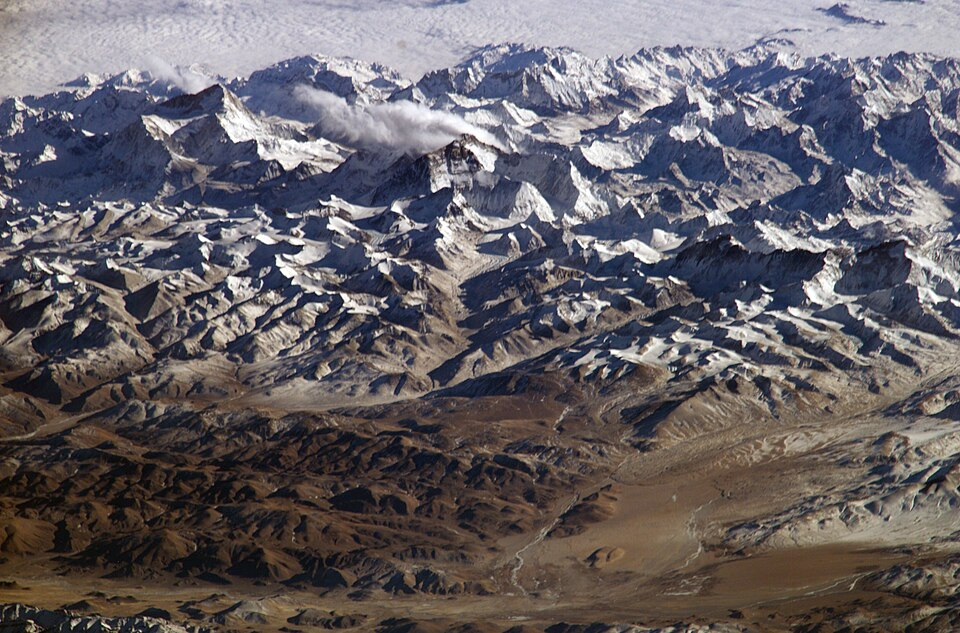
\includegraphics[width=0.75\linewidth]{images/book1/g4-himalaya-iss.jpg}

{\small अंतरराष्ट्रीय अंतरिक्ष स्टेशन से दिखता हिमालय, तिब्बत के ऊँचे पठार से
दक्षिण की ओर देखते हुए: \omterm{def:g4:clouds-rain-snow:precipitation}{हिम} से ढकी चोटियों का एक सागर।
चित्र: नासा (सार्वजनिक डोमेन)।}
% ledger: nasa:himalaya-iss
\end{omfigure}

\section{बड़ी नदियाँ और झीलें}

\omterm{def:g4:clouds-rain-snow:precipitation}{बारिश} और पिघला हुआ \omterm{def:g4:clouds-rain-snow:precipitation}{हिम} ज़मीन पर से बहता है, धाराओं में और फिर \omterm{def:g1:landscapes-around-us:water}{नदियों} में
मिलता है, और \omterm{def:g1:landscapes-around-us:water}{नदियाँ} पानी को नीचे \omterm{def:g2:water-on-earth:ocean}{समुद्र} तक ले जाती हैं। सबसे बड़ी \omterm{def:g1:landscapes-around-us:water}{नदियाँ} किसी
\omterm{def:g3:continents-and-oceans:continent}{महाद्वीप} के पूरे-पूरे क्षेत्रों का पानी बहा ले जाती हैं।

पृथ्वी की दो सबसे लंबी \omterm{def:g1:landscapes-around-us:water}{नदियाँ} अफ़्रीका की नील और दक्षिणी अमेरिका की अमेज़न
हैं। हर एक लगभग 7\,000 किलोमीटर लंबी है। सबसे लंबी कौन-सी है? इस पर कोई पक्के
तौर पर सहमत नहीं, क्योंकि यह इस पर निर्भर करता है कि तुम \omterm{def:g1:landscapes-around-us:water}{नदी} की शुरुआत कहाँ
मानते हो: उन सब छोटी धाराओं में से जो मिलकर उसे बनाती हैं, किसे उसकी असली
शुरुआत गिना जाए? 2007 में एक दल ने अमेज़न का पीछा एक और दूर के स्रोत तक किया
और कहा कि वह लगभग 6\,800 किलोमीटर लंबी है, नील से थोड़ी ज़्यादा; कई संदर्भ
पुस्तकें अब भी नील को सबसे
लंबी बताती हैं।
% ledger: natgeo:nile, natgeo:amazon-nile-2007

अमेज़न, बिना किसी संदेह के, सबसे बड़ी \omterm{def:g1:landscapes-around-us:water}{नदी} है: वह किसी भी दूसरी \omterm{def:g1:landscapes-around-us:water}{नदी} से ज़्यादा
पानी ले जाती है।
% ledger: natgeo:amazon-nile-2007

\begin{omfigure}
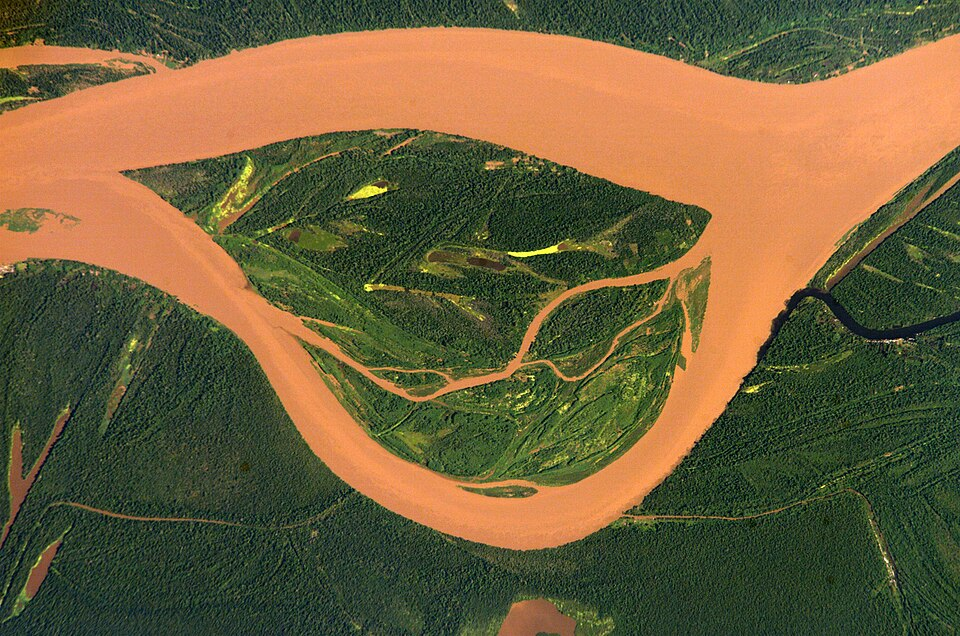
\includegraphics[width=0.6\linewidth]{images/book1/g4-amazon-iss.jpg}

{\small \omterm{def:g3:stones-pebbles-sand:sand}{कीचड़} से भूरी अमेज़न, वर्षावन के बीच बल खाती हुई, अंतरराष्ट्रीय अंतरिक्ष
स्टेशन से दिखती हुई। चित्र: नासा (सार्वजनिक डोमेन)।}
% ledger: nasa:amazon-iss
\end{omfigure}

\omterm{def:g1:landscapes-around-us:water}{झीलें} भी रिकॉर्ड तोड़ती हैं। पृथ्वी की सबसे बड़ी \omterm{def:g1:landscapes-around-us:water}{झील} कैस्पियन सागर है, यूरोप
और एशिया के बीच: वह इतनी बड़ी है कि उसे सागर कहा जाता है, पर वह हर ओर से
ज़मीन से घिरी है। वह 370\,000 वर्ग किलोमीटर से ज़्यादा में फैली है। सबसे गहरी
\omterm{def:g1:landscapes-around-us:water}{झील} रूस की बैकाल \omterm{def:g1:landscapes-around-us:water}{झील} है: कुछ जगहों पर उसका तल उसकी सतह से लगभग 2 किलोमीटर
नीचे है।
% ledger: natgeo:caspian-baikal

\section{मरुस्थल और विशाल हिम}

\omterm{def:g4:world-physical-map:physical-map}{भौतिक मानचित्र} पर दो तरह की जगहें अलग दिखती हैं, क्योंकि वहाँ लगभग कुछ नहीं
उगता: बड़े मरुस्थल, जहाँ लगभग कभी \omterm{def:g4:clouds-rain-snow:precipitation}{बारिश} नहीं होती, और विशाल
\omterm{def:g4:clouds-rain-snow:precipitation}{हिम}।

अफ़्रीका के उत्तर में सहारा पृथ्वी का सबसे बड़ा गरम मरुस्थल है। वह लगभग
पचासी लाख (साढ़े आठ मिलियन) वर्ग किलोमीटर में फैला
है। पूरा अफ़्रीका लगभग 3 करोड़ वर्ग किलोमीटर में फैला है, इसलिए सहारा \omterm{def:g3:continents-and-oceans:continent}{महाद्वीप} के
एक-चौथाई से थोड़ा ज़्यादा है: $\frac{1}{4}$ से ज़्यादा, पर
$\frac{1}{3}$ से कम।
% ledger: natgeo:sahara, data:etopo1

विशाल \omterm{def:g4:clouds-rain-snow:precipitation}{हिम} \omterm{def:g3:continents-and-oceans:poles}{दक्षिणी ध्रुव} के चारों ओर अंटार्कटिका को, और अटलांटिक के सुदूर उत्तर
में ग्रीनलैंड के ज़्यादातर हिस्से को ढकता है। वहाँ हज़ारों वर्षों का \omterm{def:g4:clouds-rain-snow:precipitation}{हिम} जमा
होकर बर्फ़ की एक मोटी परत बन गया है। \omterm{def:g4:world-physical-map:physical-map}{भौतिक मानचित्र} पर उनके रंग ऊँची ज़मीन के रंग हैं,
क्योंकि बर्फ़ की ऊपरी सतह \omterm{def:g4:world-physical-map:altitude}{समुद्र तल} से बहुत ऊपर है।

\section{सबसे ऊँचा और सबसे गहरा}

\omterm{def:g4:world-physical-map:physical-map}{भौतिक मानचित्र} पृथ्वी की सतह का आकार दिखाता है, पर वह इतना छोटा है कि
चरम सीमाओं को छिपा देता है। आओ, उन्हें पैमाने पर एक-दूसरे के बगल में रखें।

\begin{omfigure}
\begin{tikzpicture}[x=1cm, y=0.32cm, font=\small]
  % sea level
  \fill[omHypsSeaA] (0,0) rectangle (9,-11.5);
  \fill[omHypsSeaD!80] (4.6,-11.5) -- (4.6,-11.0) -- (5.0,-10.98) -- (5.4,-11.0) -- (5.4,-11.5) -- cycle;
  \draw[black!60] (-0.2,0) -- (9.2,0);
  \node[anchor=west, font=\scriptsize] at (9.25,0) {समुद्र तल, 0\,मी};
  % height scale
  \draw[black!60] (0,-11.5) -- (0,10);
  \foreach \h in {-10,-8,...,8} {
    \draw[black!60] (-0.1,\h) -- (0,\h);
    \node[anchor=east, font=\scriptsize] at (-0.12,\h) {\h\,किमी};
  }
  % ocean floor and trench
  \fill[brown!45] (0.05,-11.5) -- (0.05,-3.7) -- (3.2,-3.7) -- (4.4,-6) -- (4.9,-10.98) -- (5.1,-10.98)
    -- (5.6,-6) -- (6.4,-3.7) -- (9,-3.7) -- (9,-11.5) -- cycle;
  \node[font=\scriptsize, align=center] at (2.0,-5.3) {महासागर का तल,\\लगभग 3\,700\,मी गहरा};
  \node[font=\scriptsize, anchor=west, align=left] at (5.6,-9.4) {सबसे गहरा बिंदु:\\चैलेंजर गर्त,\\लगभग 11\,000\,मी};
  % Everest
  \fill[black!35] (6.6,0) -- (7.6,8.85) -- (8.6,0) -- cycle;
  \fill[white, draw=black!45, line width=0.3pt] (7.35,6.6) -- (7.6,8.85) -- (7.85,6.6) -- (7.6,7.1) -- cycle;
  \node[font=\scriptsize, align=center, anchor=south] at (7.6,8.95) {माउंट एवरेस्ट, 8\,849\,मी};
  % cirrus clouds band
  \draw[black!45, line width=0.6pt] (1.0,9.0) .. controls (1.6,9.5) and (2.2,9.1) .. (2.8,9.6);
  \draw[black!45, line width=0.6pt] (1.2,8.3) .. controls (1.8,8.8) and (2.4,8.4) .. (3.0,8.9);
  \node[font=\scriptsize, align=center] at (2.0,7.2) {ऊँचे बादल\\(पक्षाभ मेघ)};
  % a village
  \fill[black!60] (2.2,1.5) rectangle (2.45,1.75);
  \node[font=\scriptsize, anchor=west] at (2.5,1.6) {एक पहाड़ी गाँव, 1\,500\,मी};
\end{tikzpicture}

{\small \omterm{def:g2:water-on-earth:ocean}{महासागर} के सबसे गहरे बिंदु से सबसे ऊँची चोटी तक, पैमाने पर। प्रशांत
\omterm{def:g2:water-on-earth:ocean}{महासागर} का चैलेंजर गर्त \omterm{def:g2:water-on-earth:ocean}{समुद्र} के नीचे उससे ज़्यादा गहरा है जितना माउंट एवरेस्ट
उसके ऊपर उठा है। मान: एवरेस्ट 8\,849\,मी; चैलेंजर गर्त लगभग 11\,000\,मी;
\omterm{def:g2:water-on-earth:ocean}{महासागर} का औसत तल लगभग
3\,700\,मी।}
\label{fig:g4:world-physical-map:extremes}
% ledger: tht:everest, usgs:trench-depth, nos:ocean-depth, wmo:cloud-levels
\end{omfigure}

\begin{example}[गहराई में एवरेस्ट]\label{ex:g4:world-physical-map:everest-in-deep}
अगर हम माउंट एवरेस्ट को उठाकर चैलेंजर गर्त के तल पर रख सकते, तो उसकी चोटी फिर
भी पानी के नीचे रहती: लगभग 11\,000 मीटर गर्त, 8\,849 मीटर \omterm{def:g1:landscapes-around-us:landform}{पर्वत} के मुक़ाबले।
2 किलोमीटर से ज़्यादा \omterm{def:g2:water-on-earth:ocean}{समुद्र} उसके ऊपर
फिर भी रहता।
% ledger: tht:everest, usgs:trench-depth
\end{example}

\section{अभ्यास}

\begin{exercise}[$\star$]\label{exo:g4:world-physical-map:1}
किसी जगह की \omterm{def:g4:world-physical-map:altitude}{ऊँचाई} क्या है? वह किस तल से नापी जाती है?
\end{exercise}

\begin{exercise}[$\star$]\label{exo:g4:world-physical-map:2}
\omterm{def:g4:world-physical-map:physical-map}{भौतिक मानचित्र} की \omterm{def:g2:drawing-to-map:legend}{संकेत-सूची} की मदद से इन रंगों वाली जगह की \omterm{def:g4:world-physical-map:altitude}{ऊँचाई} बताओ:
(क) गहरा हरा; (ख) हल्का पीला; (ग) लगभग सफ़ेद।
\end{exercise}

\begin{exercise}[$\star$]\label{exo:g4:world-physical-map:3}
ये किस \omterm{def:g3:continents-and-oceans:continent}{महाद्वीप} पर हैं: (क) एंडीज़; (ख) हिमालय; (ग) सहारा;
(घ) रॉकी \omterm{def:g1:landscapes-around-us:landform}{पर्वत}?
\end{exercise}

\begin{exercise}[$\star$]\label{exo:g4:world-physical-map:4}
पृथ्वी के सबसे ऊँचे \omterm{def:g1:landscapes-around-us:landform}{पर्वत}, सबसे बड़ी \omterm{def:g1:landscapes-around-us:water}{झील} और सबसे गहरी \omterm{def:g1:landscapes-around-us:water}{झील} के नाम बताओ।
\end{exercise}

\begin{exercise}[$\star$]\label{exo:g4:world-physical-map:5}
\omterm{def:g4:world-physical-map:physical-map}{भौतिक मानचित्र} पर तटों के पास \omterm{def:g2:water-on-earth:ocean}{समुद्र} हल्का नीला है और \omterm{def:g2:water-on-earth:ocean}{महासागरों} का बीच का हिस्सा
गहरा नीला। इससे तुम्हें \omterm{def:g2:water-on-earth:ocean}{समुद्र} की गहराई के बारे में क्या पता चलता है?
\end{exercise}

\begin{exercise}[$\star$]\label{exo:g4:world-physical-map:6}
\omterm{def:g4:world-physical-map:physical-map}{भौतिक मानचित्र} पर अंटार्कटिका और ग्रीनलैंड ऊँची ज़मीन जैसे रंग में क्यों
रँगे हैं?
\end{exercise}

\begin{exercise}[$\star\star$]\label{exo:g4:world-physical-map:7}
सबसे नीचे से सबसे ऊँचे के क्रम में लगाओ: एक \omterm{def:g2:water-on-earth:ocean}{समुद्र} \omterm{def:g1:landscapes-around-us:water}{तट}; 1\,500 मीटर पर एक
गाँव; माउंट एवरेस्ट की चोटी; चैलेंजर गर्त का तल; \omterm{def:g2:water-on-earth:ocean}{महासागर} का औसत
तल।
\end{exercise}

\begin{exercise}[$\star\star$]\label{exo:g4:world-physical-map:8}
हम पक्के तौर पर क्यों नहीं कह सकते कि नील सबसे लंबी \omterm{def:g1:landscapes-around-us:water}{नदी} है या अमेज़न?
\end{exercise}

\begin{exercise}[$\star\star$]\label{exo:g4:world-physical-map:9}
अफ़्रीका लगभग 3 करोड़ वर्ग किलोमीटर में फैला है। उसका एक-चौथाई कितना है?
एक-तिहाई? सहारा लगभग पचासी लाख वर्ग किलोमीटर में फैला है: क्या वह अफ़्रीका के
एक-चौथाई से ज़्यादा है या कम? एक-तिहाई से ज़्यादा या कम?
\end{exercise}

\begin{exercise}[$\star\star$]\label{exo:g4:world-physical-map:10}
एक \omterm{def:g1:landscapes-around-us:landform}{पहाड़ी} झोंपड़ी 2\,500 मीटर पर है, और उसके नीचे एक \omterm{def:g1:landscapes-around-us:water}{झील} 1\,000 मीटर पर। झोंपड़ी
\omterm{def:g1:landscapes-around-us:water}{झील} से कितने मीटर ऊँची है? \omterm{def:g4:world-physical-map:physical-map}{भौतिक मानचित्र} पर उनके रंग कौन-से हैं?
\end{exercise}

\begin{exercise}[$\star\star\star$]\label{exo:g4:world-physical-map:11}
एक हवाई जहाज़ \omterm{def:g4:world-physical-map:altitude}{समुद्र तल} से 10 किलोमीटर ऊपर उड़ता है। क्या वह माउंट एवरेस्ट से
ऊँचा है? कितने मीटर? अगर वह चैलेंजर गर्त के ऊपर से उड़े, तो वह गर्त के तल से
कितना ऊपर होगा (गर्त के लिए 11\,000 मीटर लो)?
\end{exercise}
